\documentclass[tikz, border=2pt]{standalone}

\usepackage[dvipsnames]{xcolor}
\usetikzlibrary{arrows.meta, positioning}

\newcommand{\PredWR}{\mathsf{PredWR}}
\newcommand{\PredRW}{\mathsf{PredRW}}

\begin{document}
  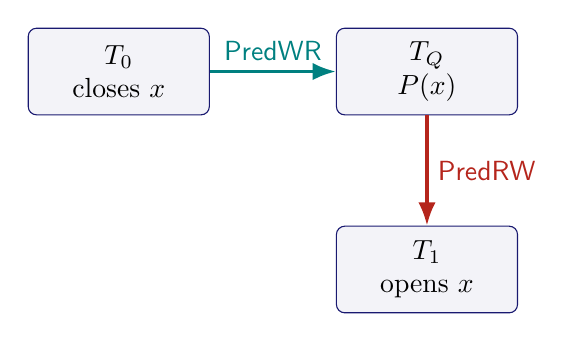
\begin{tikzpicture}[
      >=Latex,
      font = \normalsize,
      tx/.style={
        draw = MidnightBlue,
        rounded corners = 3pt,
        fill = MidnightBlue!5,
        minimum width = 23mm,
        minimum height = 11mm,
        align = center,
      },
    ]
    \node[tx] (w) {$T_0$\\closes $x$};
    \node[tx, right = 16mm of w] (q) {$T_Q$\\$P(x)$};
    \node[tx, below = 14mm of q] (u) {$T_1$\\opens $x$};
    \draw[-Latex, very thick, teal] (w) -- node[above] {$\PredWR$} (q);
    \draw[-Latex, very thick, BrickRed] (q) -- node[right] {$\PredRW$} (u);
  \end{tikzpicture}
\end{document}
